% 建议使用 XeLaTeX 或 LuaLaTeX 编译(中文与公式支持更佳)
\documentclass[UTF8,zihao=-4]{ctexart}

\usepackage[a4paper,margin=2.5cm]{geometry}
\usepackage{amsmath, amssymb, amsthm}
\usepackage{bm}
\usepackage{hyperref}
\usepackage{graphicx}
\usepackage{caption}
\usepackage{listings}
\usepackage{xcolor}
\usepackage{float}
\usepackage{placeins}
\graphicspath{{figures/}}

\lstdefinestyle{code}{
  basicstyle=\ttfamily\small,
  numbers=left,
  numberstyle=\tiny,
  numbersep=8pt,
  keywordstyle=\color{blue},
  commentstyle=\color{teal!70!black},
  stringstyle=\color{orange!70!black},
  showstringspaces=false,
  breaklines=true,
  frame=single,
  framerule=0.3pt,
  rulecolor=\color{black!15}
}
\lstset{style=code}

\title{异步优势演员-评论家(A3C):原理、公式、应用与实战}
\author{}
\date{\today}

\begin{document}
\maketitle

\section{引言}
异步优势演员-评论家(Asynchronous Advantage Actor-Critic,A3C)通过多个并行工作线程采样、更新共享的策略与价值网络,避免经验回放带来的相关性问题。异步更新提升探索多样性,并充分利用多核 CPU 资源,是早期深度强化学习中的重要里程碑。

\section{原理与公式}
\subsection{多工作线程目标}
每个工作线程从全局参数 \((\theta, w)\) 拷贝本地副本 \((\theta', w')\),采集长度为 \(n\) 的轨迹,并计算多步优势:
\begin{equation}
A_t = \sum_{k=0}^{n-1} \gamma^k r_{t+k+1} + \gamma^n V_w(s_{t+n}) - V_w(s_t).
\end{equation}
本地累积梯度后再应用到全局参数。

\subsection{异步更新}
策略与价值的梯度分别为:
\begin{align}
\nabla_\theta J &\approx \sum_t \nabla_\theta \log \pi_\theta(a_t\mid s_t) A_t + \beta \nabla_\theta H[\pi_\theta(\cdot\mid s_t)],\\
\nabla_w L_V &\approx \sum_t \partial_w \frac{1}{2} A_t^2,
\end{align}
其中 \(\beta\) 控制熵正则强度。计算完成后,工作线程将梯度异步地加到全局网络,再同步参数副本。

\subsection{稳定性考量}
异步执行会增加梯度噪声,需要通过较小的 rollout 长度、梯度裁剪、一致的学习率以及共享 RMSprop 统计量来维持稳定。适度的熵系数有助于避免线程过早收敛到同一策略。

\section{应用与技巧}
\begin{itemize}
  \item \textbf{CPU 友好训练}:无需大型 replay buffer,即可充分利用多核服务器。
  \item \textbf{稀疏奖励}:多线程可并行探索不同轨迹,提高成功率。
  \item \textbf{离散/连续控制}:可扩展到高维 CNN 编码器或高斯策略。
  \item \textbf{实用建议}:定期同步参数,针对每个线程设置学习率退火,监控梯度范数以防发散。
\end{itemize}

\section{Python 实战}
脚本 \texttt{gen\_a3c\_figures.py} 模拟三个异步线程在“悬崖”网格世界中训练,使用多步优势估计更新共享策略与价值表,并输出汇总回报及策略概率热力图。
\begin{lstlisting}[language=Python,caption={脚本 gen_a3c_figures.py 片段}]
for worker in range(num_workers):
    states, actions, rewards = collect_rollout(theta_local[worker], V_local[worker])
    advantages = compute_n_step_advantages(states, rewards, V_global)
    grad_theta, grad_V = accumulate_gradients(states, actions, advantages)
    theta_global += actor_lr * grad_theta
    V_global += critic_lr * grad_V
\end{lstlisting}

\section{实验结果}
\begin{figure}[H]
  \centering
  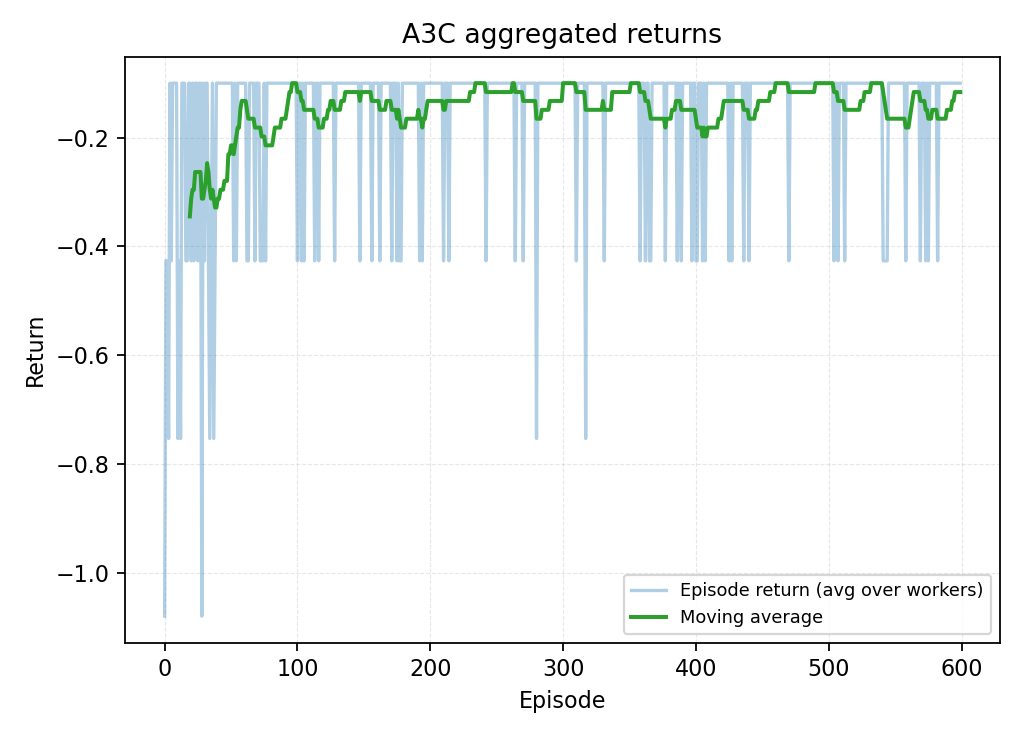
\includegraphics[width=0.8\linewidth]{a3c_returns.png}
  \caption{多个线程异步更新后的回报曲线}
  \label{fig:a3c_returns_cn}
\end{figure}

\begin{figure}[H]
  \centering
  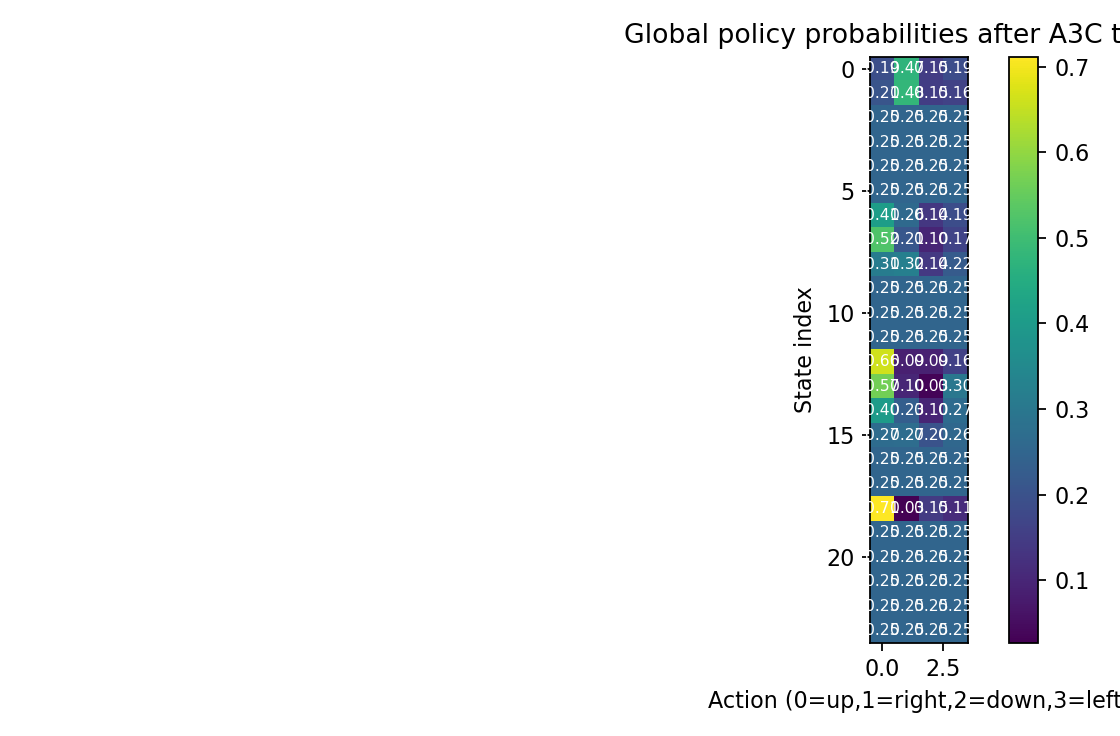
\includegraphics[width=0.82\linewidth]{a3c_policy_heatmap.png}
  \caption{最终策略的状态-动作概率热力图}
  \label{fig:a3c_policy_heatmap_cn}
\end{figure}

\FloatBarrier
\section{总结}
A3C 结合多步优势估计与异步线程,实现无需回放缓冲的稳定在线策略学习。合理选择 rollout 长度、熵系数与优化器可平衡梯度噪声与收敛速度。示例展示了多线程带来的收益以及策略概率如何集中在安全路径上。

\end{document}